\documentclass[border=8pt]{standalone}

\usepackage{pgfplots}
\pgfplotsset{compat=1.18}

% ----------------------------------------------------------
%  Cornell Palette
% ----------------------------------------------------------
\definecolor{CornellRed}   {RGB}{179, 27,  27}
\definecolor{CornellDark}  {RGB}{ 91,  0,   0}
\definecolor{CornellMid}   {RGB}{140, 20,  20}
\definecolor{CornellAccent}{RGB}{220,170,170}
\definecolor{CornellLight} {RGB}{250,238,238}
\definecolor{CornellGray}  {RGB}{ 84, 88,  90}
\definecolor{LoRABlue}     {RGB}{ 60,100,165}
\definecolor{NumGreen}     {RGB}{ 30,120, 60}
\definecolor{BodyBg}       {RGB}{255,255,255}
\definecolor{TableShade}   {RGB}{253,238,238}

\begin{document}
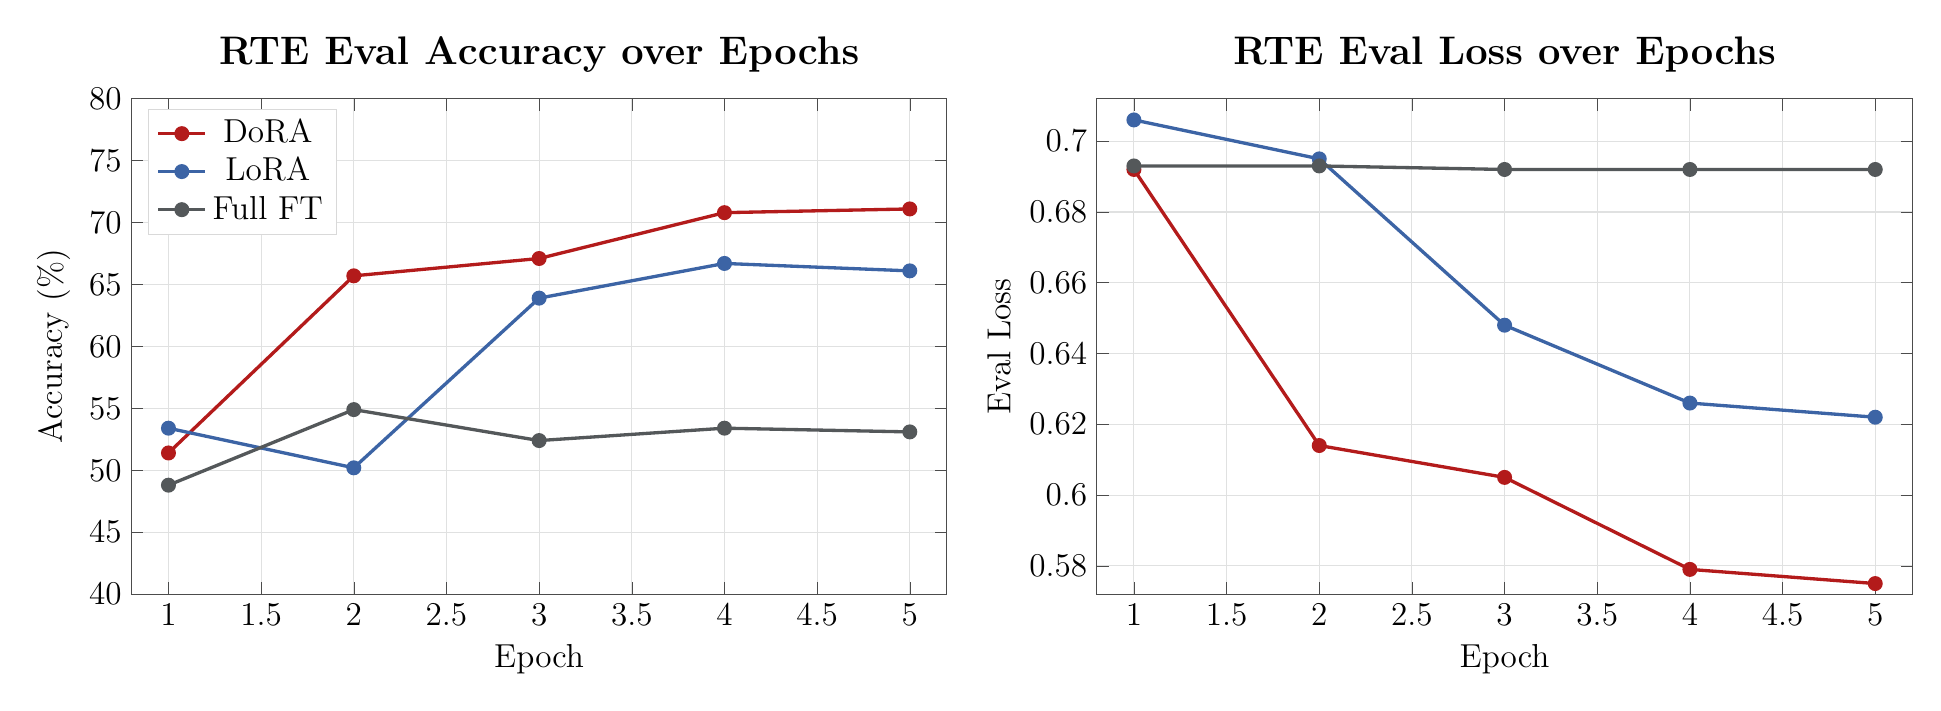
\begin{tikzpicture}

\begin{axis}[
    name=accuracy,
    width=4.7in,
    height=3.1in,
    title={RTE Eval Accuracy over Epochs},
    title style={font=\bfseries\Large},
    xlabel={Epoch},
    ylabel={Accuracy (\%)},
    label style={font=\large},
    tick label style={font=\large},
    xmin=0.8,
    xmax=5.2,
    ymin=40,
    ymax=80,
    xtick={1,1.5,2,2.5,3,3.5,4,4.5,5},
    ytick={40,45,50,55,60,65,70,75,80},
    grid=major,
    major grid style={draw=CornellGray!18},
    axis line style={draw=black!70},
    tick style={draw=black!70},
    legend style={
        at={(0.02,0.98)},
        anchor=north west,
        draw=black!15,
        fill=BodyBg,
        font=\large
    },
]

\addplot[
    CornellRed,
    very thick,
    mark=*,
    mark size=2.1pt,
] coordinates {
    (1,51.4) (2,65.7) (3,67.1) (4,70.8) (5,71.1)
};
\addlegendentry{DoRA}

\addplot[
    LoRABlue,
    very thick,
    mark=*,
    mark size=2.1pt,
] coordinates {
    (1,53.4) (2,50.2) (3,63.9) (4,66.7) (5,66.1)
};
\addlegendentry{LoRA}

\addplot[
    CornellGray,
    very thick,
    mark=*,
    mark size=2.1pt,
] coordinates {
    (1,48.8) (2,54.9) (3,52.4) (4,53.4) (5,53.1)
};
\addlegendentry{Full FT}

\end{axis}

\begin{axis}[
    at={(accuracy.east)},
    anchor=west,
    xshift=0.75in,
    width=4.7in,
    height=3.1in,
    title={RTE Eval Loss over Epochs},
    title style={font=\bfseries\Large},
    xlabel={Epoch},
    ylabel={Eval Loss},
    label style={font=\large},
    tick label style={font=\large},
    xmin=0.8,
    xmax=5.2,
    ymin=0.572,
    ymax=0.712,
    xtick={1,1.5,2,2.5,3,3.5,4,4.5,5},
    ytick={0.58,0.60,0.62,0.64,0.66,0.68,0.70},
    grid=major,
    major grid style={draw=CornellGray!18},
    axis line style={draw=black!70},
    tick style={draw=black!70},
]

\addplot[
    CornellRed,
    very thick,
    mark=*,
    mark size=2.1pt,
] coordinates {
    (1,0.692) (2,0.614) (3,0.605) (4,0.579) (5,0.575)
};

\addplot[
    LoRABlue,
    very thick,
    mark=*,
    mark size=2.1pt,
] coordinates {
    (1,0.706) (2,0.695) (3,0.648) (4,0.626) (5,0.622)
};

\addplot[
    CornellGray,
    very thick,
    mark=*,
    mark size=2.1pt,
] coordinates {
    (1,0.693) (2,0.693) (3,0.692) (4,0.692) (5,0.692)
};

\end{axis}

\end{tikzpicture}
\end{document}
